\title{Assignment 1: CS 763, Computer Vision}
\author{Sasank Chilamkurthy\\ Tharun Kumar Reddy\\ Rajeev Puppala}

\documentclass[11pt]{article}

\usepackage{amsmath}
\usepackage{amssymb}
\usepackage{hyperref}
\usepackage{ulem}
\usepackage{fancyvrb}
\usepackage{todonotes}

\usepackage[margin=0.5in]{geometry}
\usepackage{subfig}

\newcommand{\norm}[1]{\left\lVert#1\right\rVert}
\newcommand{\tr}{\operatorname{trace}}

\begin{document}
\maketitle

\begin{enumerate}
\item \textit{In class, we have seen image formation on a flat screen (i.e. image plane) with a pinhole camera. Now suppose the screen was wrapped on the surface of a sphere and hence, the 3D points were projected onto a spherical surface. Derive a relationship between the coordinates of a 3D point $P = (X,Y,Z)$ and its image on such a screen (both in camera coordinate system). If you had to calibrate this sort of a system, what are the additional intrinsic parameters of the camera as compared to the case of an image plane ? \textsf{[4 points]}}
\begin{itemize}
	\item[Ans.] Let origin be the pinhole and $(0,0,c)$ be the centre and $r$ be the radius of the screen sphere. Intersection of line passing through the pinhole and the point $P = (X,Y,Z)$ and screen sphere is the requried projection.
	Since general point on the sphere can be parametrized as $(r\sin{\theta}\cos{\phi}, r\sin{\theta}\sin{\phi}, c+r\cos{\theta})$,
	\[	\frac{r\sin{\theta}\cos{\phi}}{X} = \frac{r\sin{\theta}\sin{\phi}}{Y} = \frac{c+r\cos{\theta}}{Z}
	\]
	From first part of the equation,
	\begin{align}
		\frac{r\sin{\theta}\cos{\phi}}{X} &= \frac{r\sin{\theta}\sin{\phi}}{Y}\\
		\tan{\phi} &= Y/X  \\
		\phi &= \tan ^{-1}{\frac{Y}{X}} \\
		\sin{\phi} &= \frac{Y}{\sqrt{X^2+Y^2}}
	\end{align}

	using this in the second part of the equation,
	\begin{align}
		\frac{r\sin{\theta}\sin{\phi}}{Y} &= \frac{c+r\cos{\theta}}{Z}\\
		\frac{r\sin{\theta}}{\sqrt{X^2+Y^2}} &= \frac{c+r\cos{\theta}}{Z}		 
	\end{align}
	Let $K=\sqrt{X^2+Y^2}$

	\begin{align}
	 Zr\sin{\theta}&=K(c+r\cos{\theta})\\
	 r(Z\sin{\theta}-K\cos{\theta})&=Kc	  
	\end{align}
	Divide either side by $\sqrt{Z^2+K^2}=\sqrt{X^2+Y^2+Z^2}=R$.
	We get $\sin(\theta-\cos^{-1}(\frac{Z}{R}))=\frac{Kc}{R}$. Hence,
	$\theta=\cos^{-1}(\frac{Z}{R})+\sin^{-1}(\frac{Kc}{R})$.
	%\todo[inline]{complete these equations}
We've thus determined $\theta$ and $\phi$ in terms of the r,c and X,Y,Z.

Therefore the image of the point $(X,Y,Z)$ on the image sphere is 
\[
(r\sin{\theta}\cos{\phi}, r\sin{\theta}\sin{\phi}, c+r\cos{\theta}),
\]
where $\theta=\cos^{-1}(\frac{Z}{\sqrt{X^2+Y^2+Z^2}})+\sin^{-1}(\frac{Kc}{\sqrt{X^2+Y^2+Z^2}})$ and $\phi = \tan ^{-1}{\frac{Y}{X}}$. Here, the other intrinsic parameters we are interested in are $r,c$. 
	
\end{itemize}


\item \textit{In this exercise, we will prove the orthocenter theorem pertaining to the vanishing points $Q,R,S$ of three mutually perpendicular directions $OQ, OR, OS$, where $O$ is the pinhole (origin of camera coordinate system). Let the image plane be $Z = f$. Recall that two directions $v_1$ and $v_2$ are orthogonal if $v^T_1 v_2 = 0$. One can conclude that $OS$ is orthogonal to $OR-OQ$ (why?). Also the optical axis $Oo$ (where $o$ is the optical center) is orthogonal to $OR-OQ$ (why?). Hence the plane formed by triangle $OSo$ is orthogonal to $OR-OQ$ and hence line $oS$ is perpendicular to $OR-OQ = QR$ (why?). Likewise $oR$ and $oQ$ are perpendicular to $QS$ and $RS$. Hence we have proved that the altitudes of the triangle $QRS$ are concurrent at the point $o$. QED. Now, in this proof, I considered the three perpendicular lines to be passing through $O$. How will you modify the proof if the three lines did not pass through $O$? \textsf{[4 points]}}
\begin{itemize}
\item[Ans.] $OQ, OR, OS$ are mutually perpendicular lines.\newline
Let $\bar{s},\bar{q},\bar{r}$ represent unit vectors along $OS, OQ,OR$. Therefore, $s(q-r)^{T}=0-0=0$.\newline
Hence, OS is orthogonal to $OQ-OR$. $Q,R,S$ lie on image plane $Z=f$. As $Oo$ is orthogonal to this plane. Hence, $Oo$ is orthogonal with $QR$ ,i.e., $OQ-OR$.\newline
Hence, $OS\perp(OQ-OR)$ and $Oo\perp(OQ-OR)$. $QR$ is normal to $OSo$ triangle plane.\newline
Therefore, $oS$ is $\perp QR$. Similarly $oQ \perp SR$ and $oR \perp QS$. \newline
$\implies$ $o$ is orthocentre of $\triangle QRS$ 

Even if the lines don't pass through $O$, the lines connecting vanishing points $Q,R,S$ to $O$ will be parallel to the respective original lines and are still mutually perpendicular. Hence the proof redirects to the above case.    
\end{itemize}


\item \textit{Prove that the vanishing points of three coplanar lines are collinear. \textsf{[2 points]}}
\begin{itemize}
	\item[Ans.] Consider lines 
	\[
		\frac{X-X_i}{l_i} = \frac{Y-Y_i}{m_i} = \frac{Z-Z_i}{n_i}, i = 1,2,3
	\]
	For these lines to be coplanar, it is neccesary that direction vectors of lines $v_i = (l_i,m_i,n_i)$ are coplanar or equivalently, linearly dependent. Thus,
		\[
		\begin{vmatrix}
		l_1& m_1& n_1	\\
		l_2& m_2& n_2	\\
		l_3& m_3& n_3	\\	
		\end{vmatrix}
		  = 0
		\]

	Vanishing points of these lines can be computed as
	\[
		(x_i,y_i) = \lim_{t \to \infty} \left (\frac{X_i+l_it}{Z_i+n_it},\frac{Y_i+m_it}{Z_i+n_it}\right )
				  = \left (\frac{l_i}{n_i}, \frac{m_i}{n_i}\right )
	\]

	These three points in $X-Y$ plane are collinear as 
	\[
		\begin{vmatrix}
		x_1& y_1& 1	\\
		x_2& y_2& 1	\\
		x_3& y_3& 1 \\	
		\end{vmatrix}
		  = 
		\begin{vmatrix}
		l_1/n_1& m_1/n_1& 1	\\
		l_2/n_2& m_2/n_2& 1	\\
		l_3/n_3& m_3/n_3& 1	\\	
		\end{vmatrix}
		  =		
		\begin{vmatrix}
		l_1& m_1& n_1	\\
		l_2& m_2& n_2	\\
		l_3& m_3& n_3	\\	
		\end{vmatrix}
		  = 0
	\]
	thus, proving the required statement.
\end{itemize}

\item \textit{Consider a triangle (in 3D) whose side lengths are known to you. You capture an image of this triangle and mark out the positions of its three vertices in the image (assume all vertices were visible when you took the picture). Suppose, that you knew the 3D coordinates of exactly one vertex of the triangle, in the camera coordinate system. Explain how you will determine the 3D coordinates of the other two vertices, and write down the key equations (I do not expect you to solve the equations). Assume the pixel resolution of your camera to be 1 in both directions and the optical center to be $(0,0)$. Do not assume that you knew the focal length. \textsf{[4 points]}}
\begin{itemize}
	\item[Ans.]	Let $(X_i,Y_i,Z_i), i= 1,2,3$ be the coordinates of 3 points in camera coordinate system and suppose that coordinates of the first point is known. Correspoding points in the image $(x_i,y_i) = \left(\frac{fX_i}{Z_i},\frac{fY_i}{Z_i}\right), i = 1,2,3$ are also known. We also know the distance between points, $d_{ij}$ in the camera cordiate system
	

	Equation $(x_1,y_1) = \left(\frac{fX_1}{Z_1},\frac{fY_1}{Z_1}\right)$ gives the value of $f$. From the other two equations, we get 
	\[
	(X_i,Y_i,Z_i) = \left (\frac{x_iZ_i}{f},\frac{y_iZ_i}{f},Z_i\right ), i= 2,3
	\]

	From the three equations,
	\begin{align}
		d_{12} &= \norm{(X_1,Y_1,Z_1) - \left (\frac{x_2Z_2}{f},\frac{y_2Z_2}{f},Z_2 \right )} \\
		d_{13} &= \norm{(X_1,Y_1,Z_1) - \left (\frac{x_3Z_3}{f},\frac{y_3Z_3}{f},Z_3 \right )} \\
		d_{23} &= \norm{ \left (\frac{x_2Z_2}{f},\frac{y_2Z_2}{f},Z_2 \right )  -  \left (\frac{x_3Z_3}{f},\frac{y_3Z_3}{f},Z_3 \right )}
	\end{align}
	we can find unknowns $Z_2, Z_3$ unambiguously. This will give the points $(X_i,Y_i,Z_i), i= 2,3$.
\end{itemize}


\item Consider two sets of corresponding points $\{\mathbf{p}_{1i} = (x_{1i},y_{1i})\}_{i=1}^{n}$ and $\{\mathbf{p}_{2i} = (x_{2i},y_{2i})\}_{i=1}^{n}$. Assume that each pair of corresponding points is related as follows: $\mathbf{p}_{2i} = \alpha \mathbf{R} \mathbf{p}_{1i} + \mathbf{t} + \mathbf{\eta}_i$ where $\mathbf{R}$ is an unknown rotation matrix, $\mathbf{t}$ is an unknown translation vector, $\alpha$ is an unknown scalar factor and $\mathbf{\eta}_i$ is a vector (unknown) representing noise. Explain how you will extend the method we studied in class for estimation of $\mathbf{R}$ to estimate $\alpha$ and $\mathbf{t}$ as well. Derive all necessary equations (do not merely guess the answers). \textsf{[5 points]}
\begin{itemize}
\item[Ans.] To find $\alpha,R,t$ we have to solve the optimization problem 
	\[
		\min_{\alpha,R,t} J(\alpha,R,t)= \min_{\alpha,R,t} \sum_i{\norm{\mathbf{{p}_{2i}} - \alpha R \mathbf{p}_{1i} - \mathbf{t}}}^2
		\textnormal{  s.t  } R^TR = I
	\]
	Hence, $\frac{\partial J(\alpha,R,t)}{\partial t}=0$\newline
	$\implies \sum_i 2(\mathbf{{p}_{2i}} - \alpha R \mathbf{p}_{1i} - \mathbf{t})(-1)=0$\newline
	$\implies \sum_i (\mathbf{{p}_{2i}} - \alpha R \mathbf{p}_{1i})=n\mathbf{t} $ \newline
	$\implies \mathbf{t}=  \dfrac{\sum_i (\mathbf{{p}_{2i}} - \alpha R \mathbf{p}_{1i})}{n} $ \newline
	 \begin{equation}
	\implies\mathbf{t}=  \mathbf{\bar{p}_2}-\alpha R\mathbf{\bar{p}_1}
\end{equation}	  \newline
	Substituting this in transformation function gives
	$\mathbf{p}_{2i} = \alpha \mathbf{R} \mathbf{p}_{1i} + \mathbf{\bar{p}_2}-\alpha R\mathbf{\bar{p}_1} + \mathbf{\eta}_i$.\newline Rearranging terms, we get	
	$\mathbf{p}_{2i} - \mathbf{\bar{p}_2} = \alpha \mathbf{R}( \mathbf{p}_{1i}-\mathbf{\bar{p}_1}) + \mathbf{\eta}_i$.\newline
	We can therefore define new matrices $\mathbf{\bar{P_2} }$ and $\mathbf{\bar{P_1}}$  by subtracting the respective mean vectors $\mathbf{\bar{p}_2}$ and $\mathbf{\bar{p}_1}$ from each column of $\mathbf{P_2} $ and $\mathbf{P_1}$ and the cost function transforms to  \begin{equation}
	\norm{\mathbf{\bar{P_2}} - R (\alpha \mathbf{\bar{P_1}})}_F^2
		\textnormal{  s.t  } R^TR = I
	\end{equation}\newline
		This is similar to the Procrustes problem except for the unknown factor $\alpha$. By performing SVD, we can write  $\mathbf{\bar{P_1}}\mathbf{\bar{P_2}^T}=\mathbf{U^{'}}\mathbf{S^{'}}\mathbf{V^{'^{T}}}$. Hence, $(\alpha\mathbf{\bar{P_1}})\mathbf{\bar{P_2}^T}=\mathbf{U^{'}}(\alpha\mathbf{S^{'}})\mathbf{V^{'^{T}}}$. Hence, the factor $\alpha$ doesn't effect the orthonormal matrices $\mathbf{U^{'}},\mathbf{V^{'}}$. Hence, R can be determined as a normal Procrustes problem as $R=\mathbf{V^{'}}\mathbf{U^{'^{T}}}$.\newline
		We need to now find $\alpha$.Since, we know R, we define a new matrix $\mathbf{{P_1}^{'}} = R\mathbf{\bar{P}_1}$. Hence, cost function transforms to 
		\begin{equation}		
	\norm{\mathbf{\bar{P_2}} - \alpha  \mathbf{{P_1}^{'}}}_F^2=\sum_i{\norm{\mathbf{{p}_{2i}}-\mathbf{\bar{p_2}} - \alpha R (\mathbf{p}_{1i}-\mathbf{\bar{p_1}})}}^2
				\end{equation}
Denote $\mathbf{{p}_{2i}}-\mathbf{\bar{p_2}}$ by $\mathbf{{p^{'}}_{2i}}$ and $R(\mathbf{{p}_{1i}}-\mathbf{\bar{p_1}})$ by $\mathbf{{p^{'}}_{1i}}$. 
\begin{equation}
J(\alpha,R,t)=\sum_i{\norm{\mathbf{{p^{'}}_{2i}} - \alpha\mathbf{{p^{'}}_{1i}}}}^2=\sum_i(\mathbf{{p^{'}}_{2i}} - \alpha\mathbf{{p^{'}}_{1i}})^T(\mathbf{{p^{'}}_{2i}} - \alpha\mathbf{{p^{'}}_{1i}})=K_1 \alpha^2-K_2 \alpha+K_3
\end{equation}

where $K_1=\sum_i \mathbf{{p^{'}}_{1i}}^T\mathbf{{p^{'}}_{1i}}$, $K_2=\sum_i \mathbf{{p^{'}}_{1i}}^T\mathbf{{p^{'}}_{2i}}+\sum_i \mathbf{{p^{'}}_{2i}}^T\mathbf{{p^{'}}_{1i}}=2.\sum_i \mathbf{{p^{'}}_{1i}}^T\mathbf{{p^{'}}_{2i}}$ and $K_3=\sum_i \mathbf{{p^{'}}_{2i}}^T\mathbf{{p^{'}}_{2i}}$\newline
Hence, to minimize this quadratic, we get \begin{equation}
\alpha= \frac{K_2}{2.K_1}=\frac{\sum_i \mathbf{{p^{'}}_{1i}}^T\mathbf{{p^{'}}_{2i}}}{\sum_i \mathbf{{p^{'}}_{1i}}^T\mathbf{{p^{'}}_{1i}}}
\end{equation}
Having obtained $R$ and $\alpha$ we can get $t$ from eqn. (12) given above.
\end{itemize}
\item You are given two datasets in the folder \url{http://www.cse.iitb.ac.in/~ajitvr/CS763_Spring2015/HW1/Calib_data}. The file names are Features2D\_dataset1.mat, Features3D\_dataset1.mat, Features2D\_dataset2.mat and \\ Features3D\_dataset2.mat. Each dataset contains (1) the XYZ coordinates of $N$ points marked out on a calibration object, and (2) the XY coordinates of their corresponding projections onto an image plane. Your job is to write a MATLAB program which will determine the $3 \times 4$ projection matrix $M$ such that $P_1 = MP$ where $P$ is a $4 \times N$ matrix containing the 3D object points (in homogeneous coordinates) and $P_1$ is a $3 \times N$ matrix containing the image points (in homogeneous coordinates). Use the SVD method and print out the matrix $M$ on screen (include it in your pdf file as well). Write a piece of code to verify that your computed $M$ is correct. For any one dataset, repeat the computation of the matrix $M$ after adding zero mean i.i.d. Gaussian noise of standard deviation $\sigma = 0.05 \times max_c$ (where $max_c$ is the maximum absolute value of the X,Y,Z coordinate) to every coordinate of $P$ and $P_1$ (leave the homogeneous coordinates unchanged). Comment on your results. Include these comments in your pdf file that you will submit. \textbf{Tips:} A mat file can be loaded into MATLAB memory using the `load' command. To add Gaussian noise, use the command `randn'. \textsf{[5 points]}
\begin{itemize}
	\item[Ans.] 
	These are reults for dataset 2 when noise is not added:
	\begin{Verbatim}[frame=single]
	dataset 2: 
	smallest singular value for A = 0.082374

	M =

	    0.0087    0.0011   -0.0039    0.9986
	    0.0001    0.0092    0.0005   -0.0520
	    0.0000    0.0000    0.0000    0.0027


	maximum reconstruction error =

	    2.4272
	\end{Verbatim}

	These are reults for dataset 1 when noise is not added:
	\begin{Verbatim}[frame=single]
	dataset 1: 
	smallest singular value for A = 1.7407e-15

	M =

	    0.2905    0.0532   -0.1866   -0.6283
	   -0.0881    0.3264   -0.0881   -0.6010
	    0.0002    0.0002    0.0002   -0.0021


	maxerror =

	   2.0293e-11
	\end{Verbatim}

	Now, Noise has been added to dataset1. These are the results obtained: 
	\begin{Verbatim}[frame=single]
	dataset 1: 
	adding noise
	smallest singular value of equation system = 0.13446

	M =

	    0.2728    0.0458   -0.1946   -0.6238
	   -0.1055    0.3274   -0.0880   -0.6086
	    0.0001    0.0002    0.0002   -0.0021


	maximum reconstruction error =

	   18.8168
	\end{Verbatim}

	Although $M$ looks more or less the same, reconstruction error increased quite a bit after noise is added.
\end{itemize}


\item \textit{In this exercise, you will estimate the homography between a pair of images using the method we studied in class. You should use the well-known SIFT algorithm to (1) detect salient feature points in both the images, and (2) determine pairs of matching points given the two point sets (`matching point pair' refers to points in the two images representing the same physical entity). The code for performing both these tasks is available at \url{http://www.cs.ubc.ca/~lowe/keypoints/}. We may study the internal details of how SIFT works in a separate set of lectures in class, but for this exercise, just assume this package is a magic blackbox. Now, given this set of matching pairs of points produced by the SIFT package, your job is to estimate the homography between the point sets. Write a routine of the form $\textrm{H = homography(im1,im2)}$ where $H$ is the homography matrix that will transform the first image. You will use data from the folder \url{http://www.cse.iitb.ac.in/~ajitvr/CS763_Spring2015/HW1/Homography/}. Do as follows:
\begin{enumerate}
\item Apply the homography transformation in the file `Hmodel.mat' to the image `goi1\_downsampled.jpg' using reverse warping to generate a warped image. Now estimate the homography that transforms the first image into its warped version. Apply the estimated transformation to the first image (using reverse warping) and display all three images side by side in your report. Also print the model and estimated homography matrices (make sure you normalize both so that $H(3,3) = 1$ in both cases). 
\item Determine the homography that transforms the image `goi1\_downsampled.jpg' to the second image  `goi2\_downsampled.jpg'. Warp the first image (using reverse warping) and compare it to the second. Display all three images side by side in your report. Also print the estimated homography matrix normalized so that $H(3,3) = 1$. 
\end{enumerate}
\textbf{Note:} You may not get perfect answers for the motion estimate due to errors in SIFT, but you should get a reasonable alignment. While warping, crop off the portions of the image that do not fit into the original size. You may use the nearest neighbor method for interpolation during warping. I encourage you to try out this experiment on images of planar surfaces from different viewpoints that you should take with a real camera. You will notice that the warp estimate will often be very wrong due to several incorrect matches (called as `outliers'). In a subsequent assignment, we will implement a method that will be reasonably immune to these outliers. At that point, we will attempt to mosaic together two or more pictures as well. \textsf{[6 points]}
}

\begin{itemize}
\item[Ans.] (a) 
Hest is the estimated homography matrix using SIFT.
\begin{Verbatim}
Hmodel =

    1.1283    0.0385  -57.1714
    0.0702    1.0931  -40.8860
    0.0005    0.0002    1.0000


Hest =

    1.2798    0.2091  -81.2863
    0.0727    1.3585  -86.9020
    0.0004    0.0010    1.0000
\end{Verbatim}

\begin{figure}[h]
    \centering
    \subfloat[goi1\_downsampled.jpg]{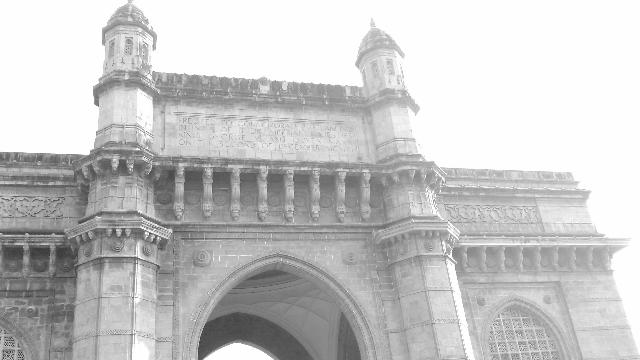
\includegraphics[width=2.5in]{goi1_downsampled.jpg}}%
    \qquad
    \subfloat[Warped using Hmodel]{{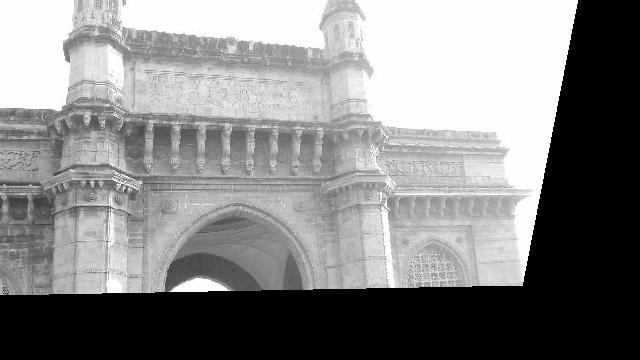
\includegraphics[width=2.5in]{goi1_downsampled_H.jpg} }}%
	\qquad
	\subfloat[Warped using Hest]{{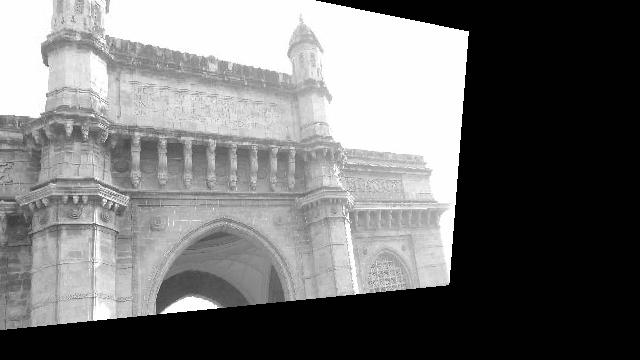
\includegraphics[width=2.5in]{goi1_downsampled_H_est.jpg} }}%
	\caption{Part - a}
\end{figure}

(b) Estimated homography  matrix between goi1\_downsampled.jpg and goi2\_downsampled.jpg is 
\begin{verbatim}
Hest =

    0.8910   -0.0359   49.5626
   -0.0650    0.9279   34.1957
   -0.0002   -0.0001    1.0000
\end{verbatim}

\begin{figure}[h]
    \centering
    \subfloat[goi1\_downsampled.jpg]{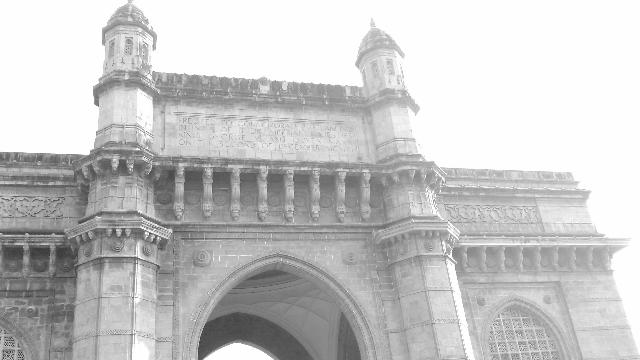
\includegraphics[width=2.5in]{goi1_downsampled.jpg}}%
    \qquad
    \subfloat[goi1\_downsampled.jpg]{{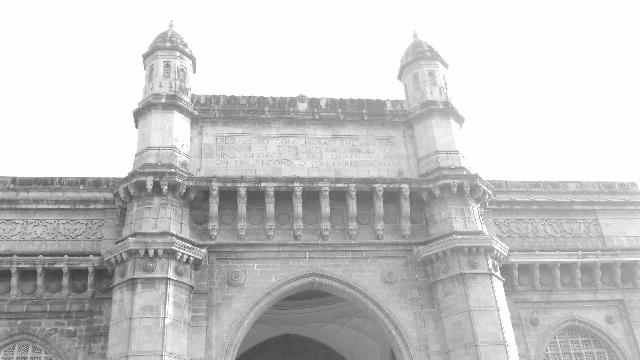
\includegraphics[width=2.5in]{goi2_downsampled.jpg} }}%
	\qquad
	\subfloat[goi1\_downsampled.jpg warped using Hest]{{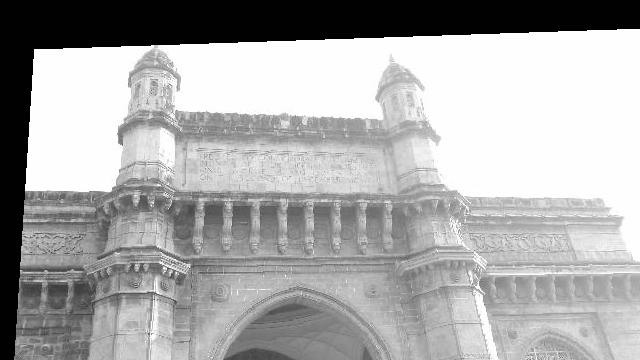
\includegraphics[width=2.5in]{goi2_downsampled_H_est.jpg} }}%
	\caption{Part - b}
\end{figure}


\end{itemize}

\end{enumerate}
\end{document}